\documentclass{article}

% if you need to pass options to natbib, use, e.g.:
%     \PassOptionsToPackage{numbers, compress}{natbib}
% before loading neurips_2020

% ready for submission
% \usepackage{neurips_2020}

% to compile a preprint version, e.g., for submission to arXiv, add add the
% [preprint] option:
%     \usepackage[preprint]{neurips_2020}

% to compile a camera-ready version, add the [final] option, e.g.:
     \usepackage[final]{neurips_2020}

% to avoid loading the natbib package, add option nonatbib:
% \usepackage[nonatbib]{neurips_2020}
\usepackage[utf8]{inputenc} % allow utf-8 input
\usepackage[T1]{fontenc}    % use 8-bit T1 fonts
\usepackage{hyperref}       % hyperlinks
\usepackage{url}            % simple URL typesetting
\usepackage{booktabs}       % professional-quality tables
\usepackage{amsfonts}       % blackboard math symbols
\usepackage{nicefrac}       % compact symbols for 1/2, etc.
\usepackage{microtype}      % microtypography
\usepackage{indentfirst}
\usepackage{amsmath}
\usepackage{graphicx}
\title{Social Media based MBTI Personality Prediction}
% The \author macro works with any number of authors. There are two commands
% used to separate the names and addresses of multiple authors: \And and \AND.
%
% Using \And between authors leaves it to LaTeX to determine where to break the
% lines. Using \AND forces a line break at that point. So, if LaTeX puts 3 of 4
% authors names on the first line, and the last on the second line, try using
% \AND instead of \And before the third author name.

\author{%
  Xinyi Cai\\
  2018533085\\
  \texttt{caixy@} \\
  \And
  Beiyuan Yang \\
  39132991 \\
  \texttt{yangby@} \\
  \And
  Wenhui Qiao \\
  57425238 \\
  \texttt{qiaowh@} \thanks{Email suffix: @shanghaitech.edu.cn} \\
}

\begin{document}

\maketitle

\begin{abstract}
It is widely accepted that people of different personality tend to post different content to social media. As s result, we tried to build a personality type predictor, based on the social media record. We applied several methods for feature extraction and classification and find some interesting results. We proposed that social media records are effective predictor, particularly accurate in some dimension, with little poorer performance on other dimension. Finally, we discuss the result and some interesting discovery.
\end{abstract}

\section{Introduction}
The Myers–Briggs Type Indicator (MBTI) is a pseudoscientific introspective self-report questionnaire indicating differing psychological preferences in how people perceive the world and make decisions. The MBTI is based on the conceptual theory, measure the personality in four dimensions. The four categories are Introversion/Extraversion, Sensing/Intuition, Thinking/Feeling, Judging/Perception. Each person is said to have one preferred quality from each category, producing 16 unique types. \\
Social media is a platform where people share their emotion or feeling, as well as recording their daily life. It could be easily proposed an assumption that what people post on social media has a correlation with their personality, i.e. people of different personality tend to have different styles in posting on social media. This paper is an attempt to invest the correlation and try to predict the personality type from the social media record. The related works is summarized in the appendix.

%\section{Related Works}
%Please refer to supplementary materials

\section{Feature Extraction}
\subsection{Dataset}
We accquired the dataset from \href{https://www.kaggle.com/datasnaek/mbti-type}{kaggle}. It contains record of social media of 8675 users, each of the data contains 50 posts on social media, as well as the type label for those 8675 users. The general distribution over these types is summarized in the graph. Readers are also welcomed to access our pre-processed data through \href{https://github.com/Martin4115/SI151_Project}{github repository}.

\subsection{Word2vec}
Before we dig into the classification tasks for these users, we must convert our text data to vector, so that it can be applied to by classification algorithm. In our project, we adapted three methods for converting vectors to text data, particularly they are one-hot coding, CBOW model and N-gram model.

\subsubsection{One-hot Coding}
Suppose we have a dictionary $W$, which contains N words, i.e.$|W|=N$. Then one-hot coding map each word to a vector $x \in \{0,1\}^N$, where $x_i=1$ if $x=W_i$, and $x_i=0$ otherwise. The picture shows a simple example of the principle of one-hot coding.\\
One possible improvement for one-hot coding is \emph{one-hot hash trick}, whose dimension is reduced by hash function. We also tried to improve the performance by applying hash function. One major shortcoming is unavoidable hash collision, which could map different values to same target.

\subsubsection{CBOW Model}
CBOW Model stands for continues bag-of-word model, which was illustrated by Xin Rong in his publication. COBW takes the words before and after the target word, to predict the target word, which is actually a way of dimension reduction. In this way, we would be able to get vectorized word representation in much lower dimension, which make it possible and efficient for future classification. The picture shows a simple structure of the network used in CBOW model. One thing to be noted is that the activation function of the hidden layer is linear, which is more similar to \emph{projection layer}.

\subsubsection{N-gram Model}
Unlike CBOW model, N-gram model intend to predict the target word based on the N word before the target words. Suppose we have a sentence, to reduce the parameter space, we adopt \emph{Markov assumption}, which state that the word's appearance only depend on the first N words before it: $$p\left(w_{1} \cdots w_{n}\right)=\prod p\left(w_{i} \mid w_{i-1} \cdots w_{1}\right) \approx \prod p\left(w_{i} \mid w_{i-1} \cdots w_{i-N+1}\right)$$. Then we could estimate the conditional probability with MLE, which takes the frequencies of words to calculate:$$p\left(w_{n} \mid w_{n-1} w_{n-2}\right)=\frac{C\left(w_{n-2} w_{n-1} w_{n}\right)}{C\left(w_{n-2} w_{n-1}\right)}$$

\subsection{Paragraph Vectorization}
So far, we have made it possible to get the feature vector from words. What we want to do is to get the feature vector for each user, which represent the feature for whole paragraph.\\
We decide to apply a naive but efficient method to compute the feature for each paragraph, which is take the weight sum of all word vectors. Suppose the paragraph as $K$ different words, we have $V = \sum_{i=1}^{K}w_iv_i$ where $v_i$ stands for the word vector for word i and $w_i = \frac{\text{\# of word i}}{\text{total length of paragraph}}$.

\section{Model for Prediction}
\subsection{Logistic Regression}

%Applying logistic regression, we get the model $Z = \theta_0 x_0 + \theta_1 x_1 +\theta_2 x_2 + ... +\theta_n x_n$. Then we use sigmoid function to transform $Z$ to $g\left( Z\right)  = \frac{1}{1+ e^{-z}}$, where $g(Z)  \in \left[0,1\right]$. Take $g(Z)$ into  the posterior probabilities, and use sum of squares as the loss function, we get $J\left( \Theta\right) = \frac{1}{n} Loss\left( h_\Theta\left( X\right), y \right) $. Repeat the update of $\theta_j^{new} = \theta_j^{old} - \alpha \frac{\partial}{\partial \theta_j}J\left( \theta\right) $ until covergence, then we got the paraments needed by the model.

Logistic regression is a statistical model that uses a logistic function to model a binary dependent variable. We firstly find the posterior probabilities of the $K$ classes via linear function in $x$, which yields $$Pr\left(G = k\mid X = x\right) = \frac{exp\left(\beta_{k0}+x^{T} \beta_{k}\right)}{1+\Sigma_{l=1}^{K-1}exp\left(\beta_{l0}+x^{T} \beta_{l}\right)},\quad k = 1,...,K-1$$ 

Then we get the log-likelihood function $l(\theta) = logPr\left(g\mid X; \theta\right) $, and use maximum likelihood estimation $\left(MLE\right)$ to estimate parameter set $\theta = \{\beta_{10},\beta_1,...,\beta_{\left(K-1\right)0},\beta_{K-1} \}$. Apply Newton-Raphson algorithm to update each $\beta$ until convergence according to $\beta_{new} \leftarrow \beta_{old} - \frac{f^{'}\left(\beta_{old}\right)}{f^{''}\left(\beta_{old}\right)}$


\subsection{Naive Bayes}
Naive Bayes is a conditional probability model, where  assumes that all the features that go into the model is independent of each other.

$$ P(Y= k|x_1x_2..x_k)= \frac{P(x_1|Y=k)*P(x_2|Y=k)...P(x_n|Y=k)*P(Y = k) }{ P(x_1)*P(x_2)...* P(X_n)}$$

In this question, to determine which MBTI type the person belongs to, we give a feature vector\\ $x = (x_1,x_2,...,x_n)$. Using Baye $ p(C_k|x) = \frac{p(C_k)p(x|C_k)}{p(x)} $. Using the "naive" conditional assumption, the joint model can be expressed as $p(C_k|x_1x_2...x_n) = p(C_k)\prod_{i-1}^n p(x_1|C_k)$ 

\subsection{Support Vector  Regression}

SVM is a supervised machine learning algorithm that aims to find the maximum margins between different classes by determining the weights and bias of the separating hyperplane. Given dataset \\S = ${(x_i,y_i)}_{i=1}^m $ We define our algorithm as follow:
$$ min_{w,\xi_1,...\xi_m}||w||^2 + C\sum_{i=1}^m \xi_i \quad \emph{s.t} \ for \ all \ i, \ y_i w x_i \ge 1 - \xi_i, \xi_i \ge 0 $$
We can implement this algorithm with kernel which identifies boundaries in a high-dimensional feature space, thus  we can split the training set into labeled 16 categories.
\subsection{Neural Network}
\subsubsection{Simple Sequential Network}
The first attempt we tried is to classify the data with sequential neural network. It has two hidden layers, which consist of 32 unit, and take RELU as activation function. In the output layer, we use sigmoid function to output the classification result between $(0,1)$. The structure is shown in the picture \ref{fig:result1}.
\subsubsection{LSTM Recurrent Network}
During the experiment, we find that the simple sequential network suffered from gradient vanish problem, which limit its performance. To overcome it, we import the long-short term memory recurrent network, which was originally proposed by Sepp Hochreiter and Jürgen Schmidhuber in 1997. It gains an ability to bring information between time slots. Save the information for later using, to prevent the earlier signal from disappearing while processing.\\
The structure of LSTM net we used was shown in the picture \ref{fig:result1}. It is considered to be a effective way to deal with the problem of gradient vanishing.

\begin{figure}[h]
	\centering
	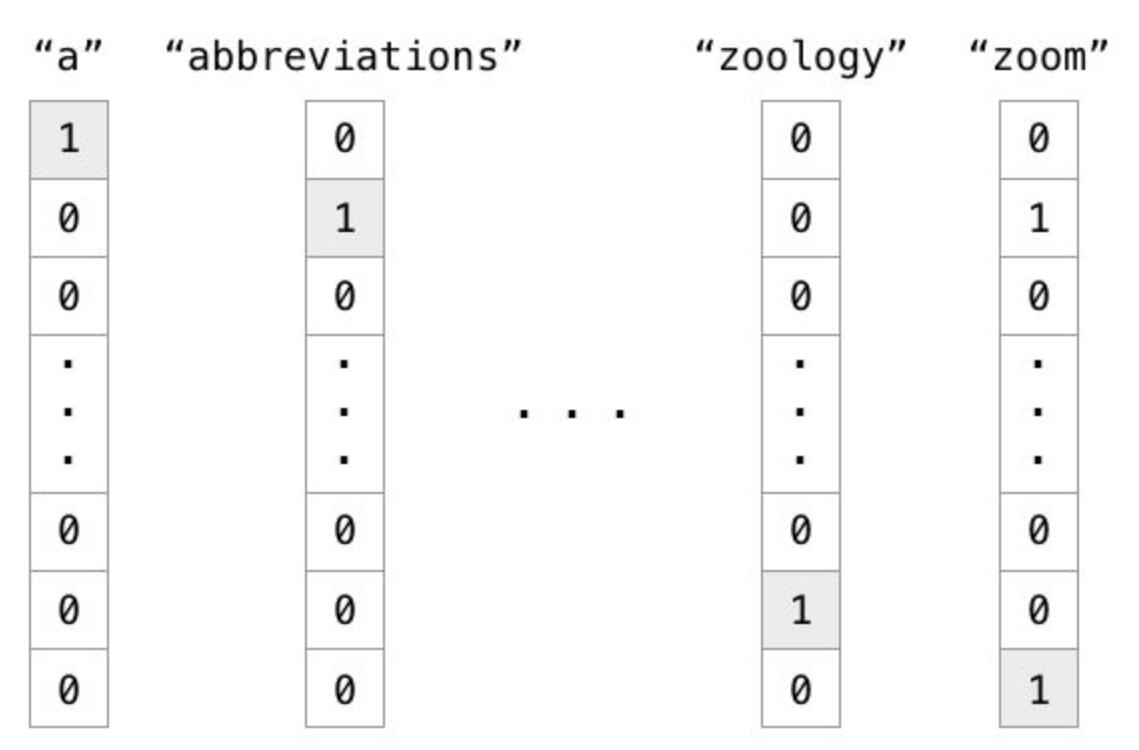
\includegraphics[width=4cm]{fig/oneHot.jpg}
	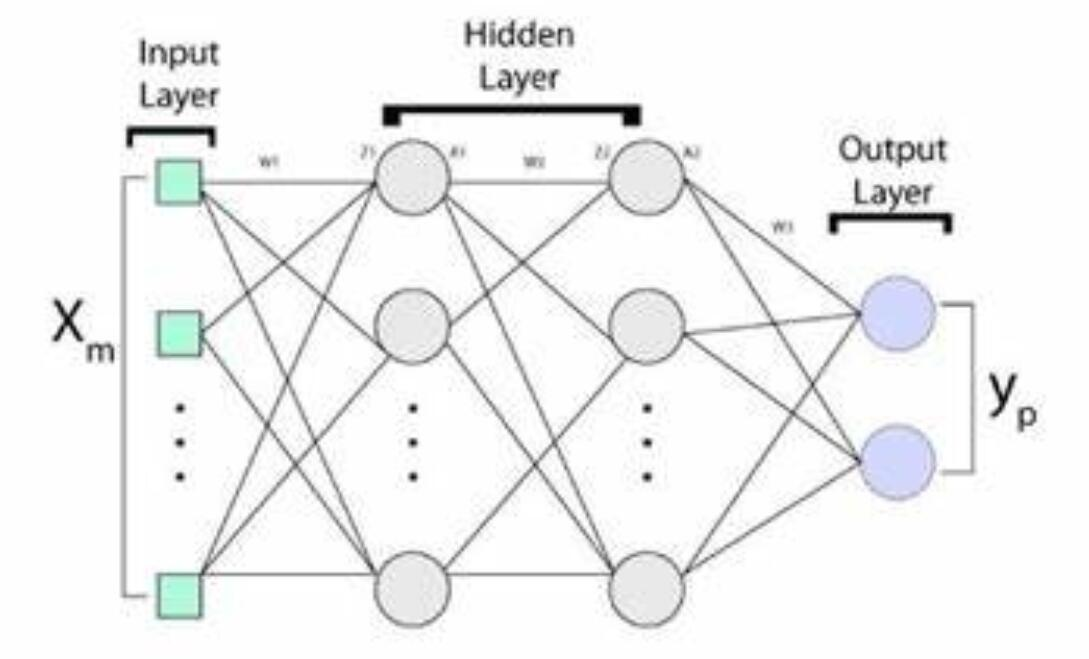
\includegraphics[width=4cm]{fig/snn.jpg}
	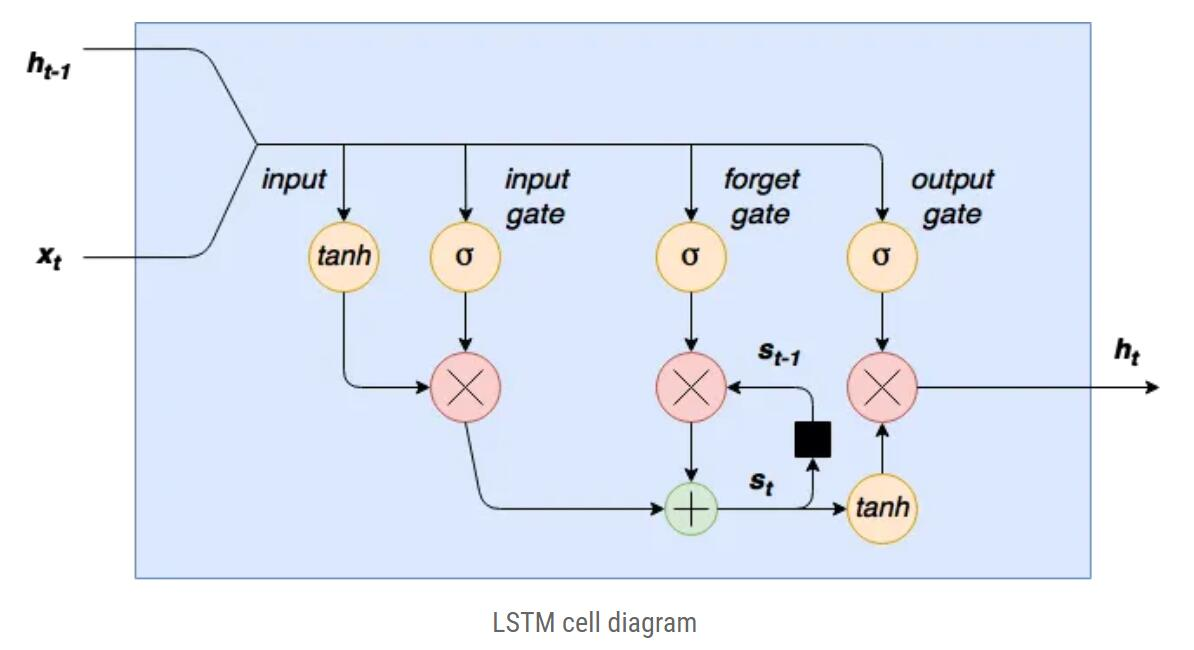
\includegraphics[width=4cm]{fig/lstm.jpg}
	\caption{\emph{Left:} One-hot coding. \emph{Middle:} Sequential neural Network. \emph{Right:} LSTM Network.}
	\label{fig:result1}
\end{figure}

\subsection{XGBoost}

XGboost is an improvement of gradient lifting algorithm. Newton method is used to solve the extreme value of loss function. It applies Taylor expansion to the loss function, only keep the first two orders, and the regularization term is added to the loss function.\\
%Suppose we have a dataset $\mathcal{D}$, $\mathcal{D}=\left\{\left(\mathbf{x}_{i}, y_{i}\right)\right\}\left(|\mathcal{D}|=n, \mathbf{x}_{i} \in \mathbb{R}^{m}, y_{i} \in \mathbb{R}\right)$. 
The main idea is to  integrate the result of CART trees, $\hat{y}_{i}=\phi\left(\mathbf{x}_{i}\right)=\sum_{k=1}^{K} f_{k}\left(\mathbf{x}_{i}\right)$, $f_{k} \in \mathcal{F}$ where  $\mathcal{F}=\left\{f(\mathbf{x})=w_{q(\mathbf{x})}\right\}\left(q: \mathbb{R}^{m} \rightarrow T, w \in \mathbb{R}^{T}\right)$ represents the construction of each CART tree. \\
%The loss function can be expressed as $\Sigma_{i = 1}^n l(y_i,\hat{y_i})+\Sigma_{k = 1}^K\Omega(f_k) \quad where \quad  \Omega(f) = \gamma T + \frac{1}{2}\lambda \left|\left|w\right|\right| ^2$. The first part repersents the training loss and the second part represents the complexity of the trees.
We update the model by additive manner, with the loss function in $t$ turn as following: $$\hat{y}_{i}^{(t)}=\sum_{k=1}^{t} f_{k}\left(x_{i}\right)=\hat{y}_{i}^{(t-1)}+f_{t}\left(x_{i}\right)$$ $$\mathcal{L}^{(t)}=\sum_{i=1}^{n} l\left(y_{i}, \hat{y}_{i}^{(t-1)}+f_{t}\left(\mathbf{x}_{i}\right)\right)+\Omega\left(f_{t}\right), \quad where \quad  \Omega(f) = \gamma T + \frac{1}{2}\lambda \left|\left|w\right|\right| ^2$$ Here $T$ is the number of leaf nodes, $W$ is the score of leaf nodes, and $\gamma$ is a parament to controll the number of leaf nodes in order to  avoid over fitting. \\
Use Taylor expansion to expand $\mathcal{L}^{(t)}$, we get $\tilde{\mathcal{L}}^{(t)}(q)=-\frac{1}{2} \sum_{j=1}^{T} \frac{\left(\sum_{i \in I_{j}} g_{i}\right)^{2}}{\sum_{i \in I_{j}} h_{i}+\lambda}+\gamma T$. We use it to evaluate the quality of a tree, a smaller score means a higher quality. We choose to use a greedy algorithm, start with a single leaf node, iteratively split to add nodes to the tree, which can be concluded that $$\mathcal{L}_{split} = \frac{1}{2} \left[ \frac{\left( \Sigma_{i \in I_{L}} g_i\right) ^2}{\Sigma_{i \in I_{L}} h_i+\lambda} + \frac{\left( \Sigma_{i \in I_{R}} g_i\right) ^2}{\Sigma_{i \in I_{R}} h_i+\lambda} - \frac{\left( \Sigma_{i \in I} g_i\right) ^2}{\Sigma_{i \in I} h_i+\lambda} \right] - \gamma  $$

\section{Experiments and Results}
Here we listed the classification result we got. While the detail of experiment result is listed in the section 8.2, we visualize the result here.\\
For the feature extraction part, we find that the performance from different result are almost the same, so we ignore difference of ways of extracting figure. \\
Here, we compare the result from different methods for classification as well as different dimension. We find that the method of XGBoost and LSTM network get the best performance among these methods. It is also clear that some dimension like dimension 1 are more classifiable than others such as dimension 2.
\begin{figure}[h]
	\centering
	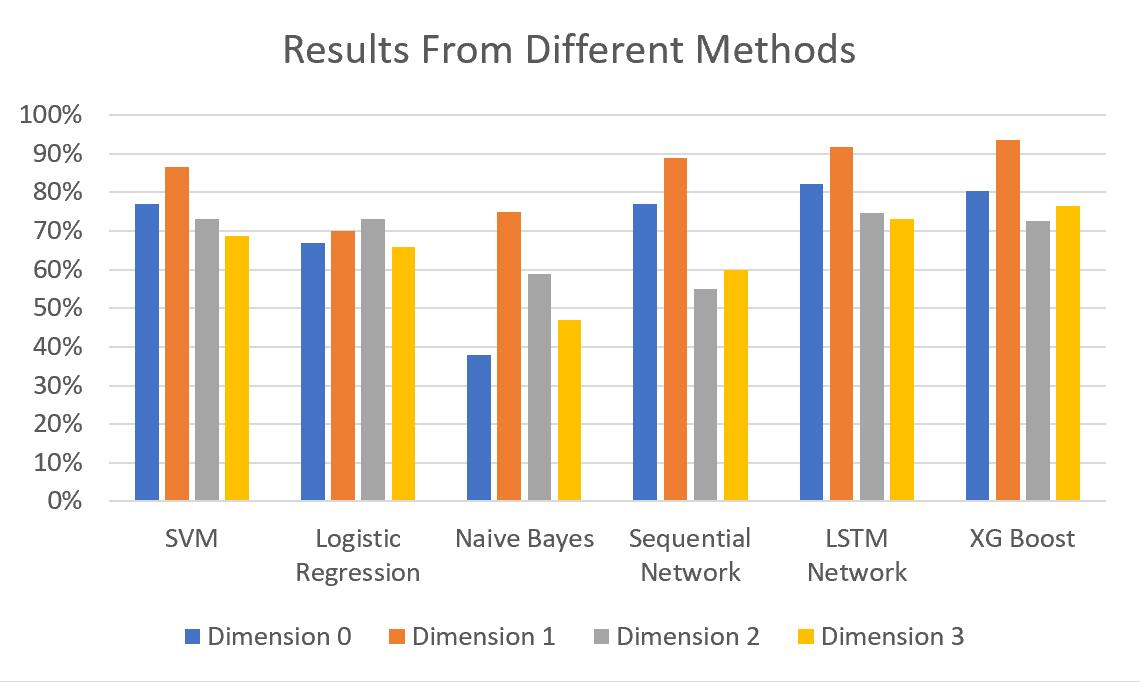
\includegraphics[width=6.3cm]{fig/result1.jpg}
	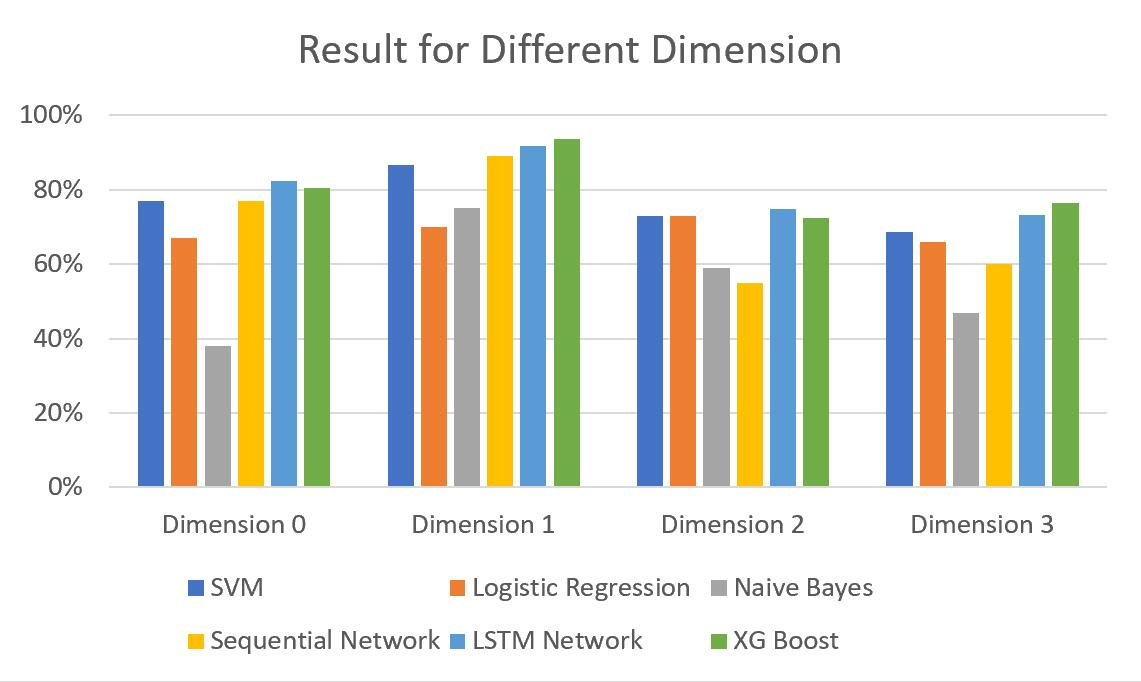
\includegraphics[width=6.3cm]{fig/result2.jpg}
	%\caption{The classification result.}
	\label{fig:result}
\end{figure}

\section{Conclusion}
Generally speaking, we can predict people's personality type from the social media records with a high probability. Specifically, it is more accurate to predict whether people are sensing and outgoing, but with less accuracy in predicting the way people act and make decision. Such discovery would lead to further psychology research to invest the principle behind it.

\section{Discussion}
During our project, we have some interesting discovery and some analysis on our method and result.
\begin{itemize}
	\item When implementing naive Bayes, we found a contradiction between the input data vectorized by word2vec and the multinomial package, since the input x of sklearn.multinomialnb must be non-negative, while the outcome of word2vec can be both positive and negative. As a result, we turned to use sklearn.GaussianNB. It is not the most suitable model, which could account for the poor performance.
	\item XGBoost is a very popular algorithm, which is used by 17 out of 25 winner projects. However, it is highly parameter dependent. Due to the limitation of computation resource, we can only adjust parameter manually. Should we achieved automatically adjust it, our performance could have been improved more.
	\item Simple sequential networks suffer a lot from gradient vanishing, which means the former information could not be applied to latter computation. Such limitation is overcome by recurrent neural network. The LSTM network managed to forget useless information and memorize crucial information, so it produced the best result among all methods.
\end{itemize}

%-------------------------------------------------------------------------



\section{Reference}


\small

[1] https://www.kaggle.com/datasnaek/mbti-type

[2]Shi X , Chen Z , Wang H , et al. Convolutional LSTM Network: A Machine Learning Approach for Precipitation Nowcasting[J]. 2015.

[3]Rong X . word2vec Parameter Learning Explained[J]. Computer ence, 2014.

[4] Darsana, M. The influence of personality and organisational culture on employee performance through organisational citizenship behaviour. Int. J. Manag. 2013, 2, 35–42. 

[5] Fernando T , Denman S , Sridharan S , et al. Soft + Hardwired Attention: An LSTM Framework for Human Trajectory Prediction and Abnormal Event Detection[J]. 2017.

[6] Brian, C. Metaprograms as a Tool for Critical Thinking in Reading and Writing, Second JALT Critical Thinking SIG forum, Kobe Convention Center, Portopia Kobe, Tokyo, 25–28 October. Available online: http://www.standinginspirit.com/wp-content/uploads/2013/10/JALT2013-Critical-Thinking-ForumHandout-Metaprograms-Explanation-Handout.pdf 


 
 
\section{Supplementar Materials}

\subsection{Related Works}
 Myers-Briggs Type Index classifies personality types in 16 ways on four dimensions, which are introverted/extroverted,  sensation/intuition, thinking/feeling and judgment /Perception[20]. Golbeck was the first few people using machine learning technology to predict personality based on Twitter comments. Komisin and Guinn then used naive bayes and SVM to predict MBTI tpye based on graduate student's writing materials and found svm had better performance compare to naive Bayes. Few years later, gray prediction models, multiple regression models, and multi-task models were applied on this field and gray prediction models performed the best among these three. Later, Tandra used five personality models and deep learning to predict MBTI personality type and found a significant improvement in performance compared to traditional algorithm using advanced algorithm. Recent years, Hernandez and Knight tried various kinds of RNN to train the model, and the result showed that LSTM gave the best prediction rate.
 
\subsubsection{Original Experiment Data}
\begin{table}[h]
	\vspace{20pt}
	\centering
	\begin{tabular}{lllll}
		\hline  
		  & Dimension 0 & Dimension 1 & Dimension 2 & Dimension 3\\
		  \hline  
		  SVM & 77\% & 86.7\% & 73\% & 68.7 \\ 
		Logistic regression & 67\% & 70\% & 73\% & 66\% \\
		Naive Bayes	& 38\%	& 75\% & 59\% &47\% \\
		Sequential Network & 77\% &	89\% & 55\% & 60\% \\
		LSTM Network & 82.30\% & 91.70\% & 74.70\% & 73.20\% \\
		XG Boost & 80.50\% & 93.60\% & 72.50\%	& 76.40\% \\
		\hline       
	\end{tabular}
	\caption{Classification Accuracy}
\label{bs}
\end{table}

\section{Contribution}
 Overall, work was well-distributed between the team members throughout the project. Qiao Wenhui implement the data-preprocess, SVM and neural network. Cai Xinyi finished the function of logistic regression and XGboost. Yang Beiyuan focused on naive Bayes, refined XGboost implementation and prepare the presentation. All three members finished this report together.

\end{document}
